\section{Fundamentação Teórica}
Neste capítulo será apresentado uma introdução sobre cada uma das partes, tecnologias e componentes, mais relevantes que possibilitaram o desenvolvimento deste projeto.

\subsection{IoT}
A Internet das Coisas (IoT, do inglês Internet of Things) surgiu a partir dos avanços em diversas áreas, como sistemas embarcados, microeletrônica, comunicação e tecnologias de sensoriamento. Ela tem atraído crescente atenção no setor industrial, devido ao seu grande potencial de aplicação em uma vasta gama de atividades humanas, sendo cada vez mais reconhecida por suas possibilidades de transformação em múltiplos setores. Em resumo, a IoT pode ser vista como uma extensão da Internet atual, permitindo que objetos do cotidiano — independentemente de sua natureza — se conectem à rede global, desde que possuam capacidade computacional e de comunicação. Essa conexão possibilita, inicialmente, o controle remoto desses objetos e, em segundo lugar, permite que eles atuem como provedores de serviços. Com isso, surgem inúmeras oportunidades no ramo industrial. \cite{santos2016internet}

\subsection{Módulo ESP32}
Para o desenvolvimento das três unidades, escolhemos o módulo "ESP WROOM-32 DevKit V1", ou apenas "ESP32", responsável pelo tratamento dos dados e pela comunicação com outros dispositivos e serviços. Este módulo é baseado no ESP32, desenvolvido pela empresa Espressif Systems, que traz embutido funções de comunicação via rádio WiFi, incluindo Bluetooth LE (Bluetooth low-energy) e um microprocessador, capaz de atender uma grande variedade de projetos \cite{gadelha2020sistema}.

Os módulos ESP32 são comercializados como placas de prototipação que possuem 32 portas digitais, sendo que 16 podem ser utilizadas como saída PWM de 12-bit e 18 entradas analógicas para conversão digital, fornecendo uma resolução de 12-bit de 0V a 3,3V \cite{espressif}.

\begin{figure}[ht]
    \centering
    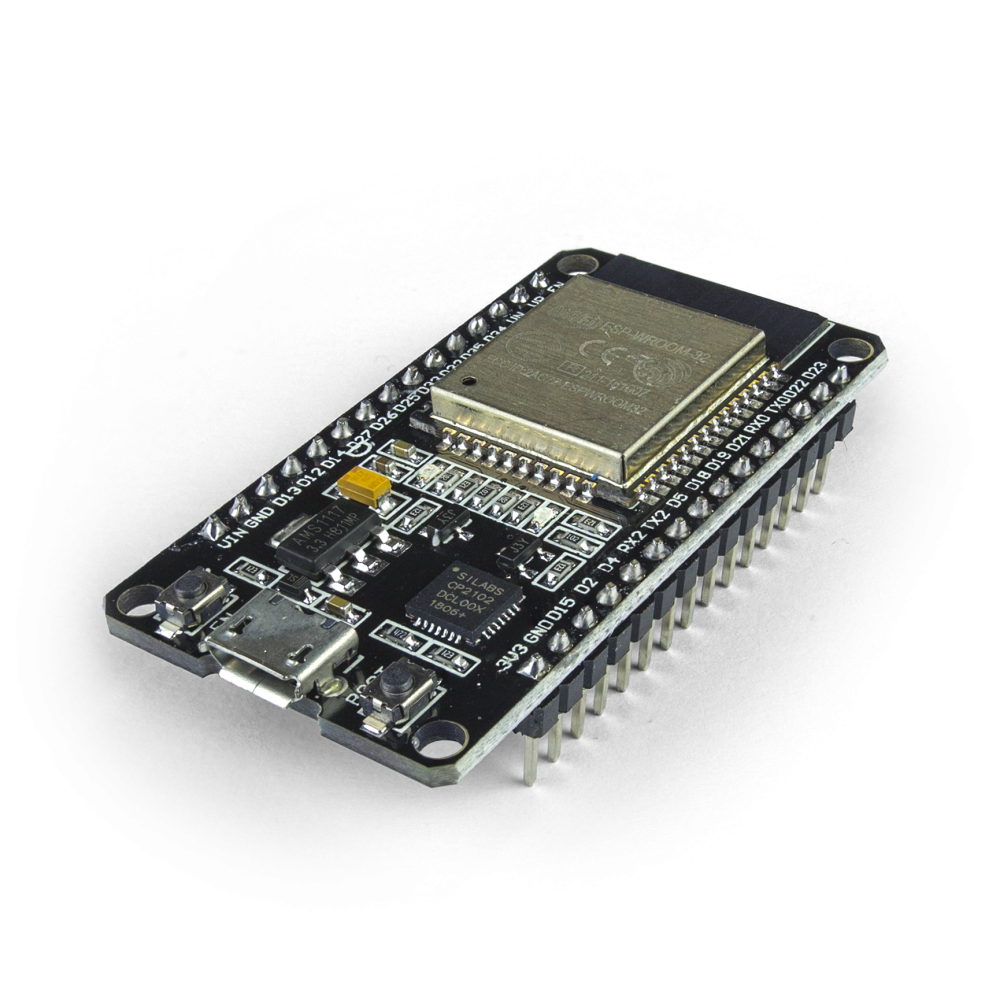
\includegraphics[width=8.5cm]{imagem/esp-wroom32.png} 
    \caption{Placa de prototipação com módulo ESP32}
    \label{fig:esp32-module}
\end{figure}

\subsection{Sensor HC-SR04}
HC-SR04 é um sensor ultrassônico de alcance que fornece a função de medição entre 2 cm a 400 cm sem contato \cite{electro}. Permite medir a distância do sensor até a superfície líquida, emitindo ondas sonoras, que são rebatidas na superfície e retorna para um receptor no equipamento \cite{tairaprototipagem}. É um componente amplamente disponível e são comercializadas unidades produzidas por diversos fabricantes diferentes.

\begin{figure}[ht]
    \centering
    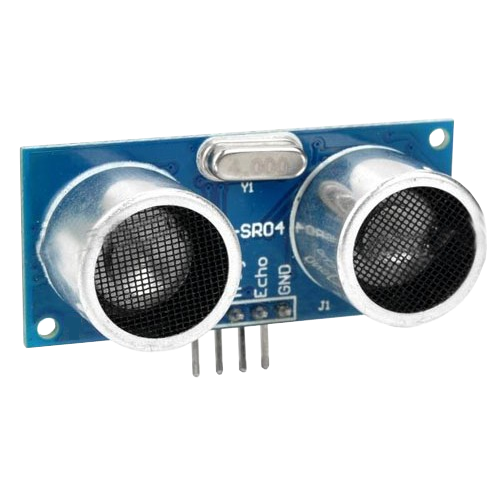
\includegraphics[width=6.5cm]{imagem/hc-sr04.png} 
    \caption{Sensor ultrassônico HC-SR04.}
    \label{fig:hc-sr04}
\end{figure}

\subsection{Mini Bomba D'água JT100}
Para as unidades de escoamento, foi utilizado uma mini bomba d’água que é usada submersa, já que seu sistema elétrico é vedado com nível de proteção IP68, além de trabalhar com tensões mais baixas entre 3V a 6V DC e com uma vazão entre 80 l/h a 120 l/h com eficiência e precisão, além de ser apropriada para prototipação com plataformas como Arduino \cite{usinainfo}. Este é também um componente amplamente disponível e são comercializadas unidades produzidas por diversos fabricantes diferentes.

\begin{figure}[ht]
    \centering
    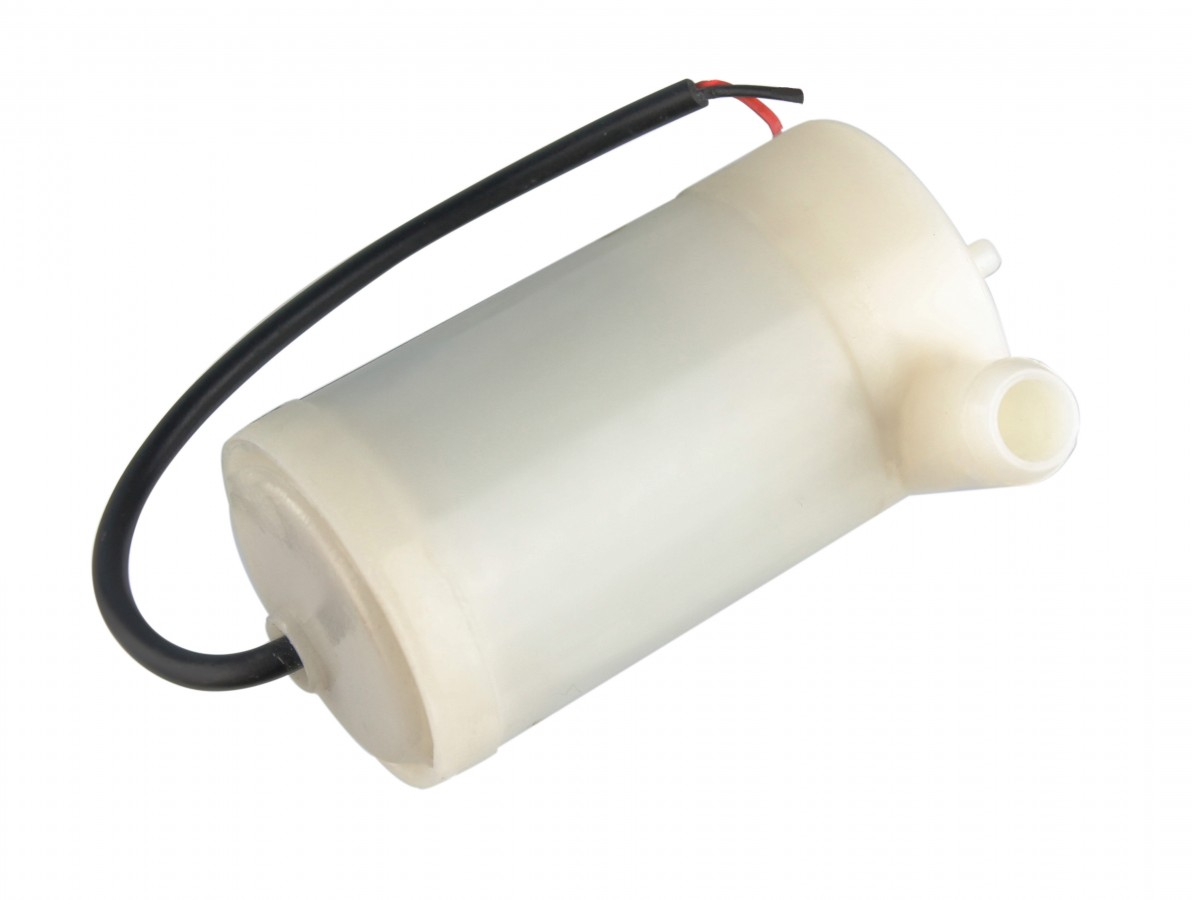
\includegraphics[width=6.5cm]{imagem/jt100.jpg} 
    \caption{Mini bomba d'água JT100.}
    \label{fig:mini-water-pump}
\end{figure}

\subsection{Transistor TIP41C NPN}
O TIP41C é um transistor NPN de alta potência podendo suportar uma tensão máxima de 100V e corrente máxima de 6A, e alta velocidade de chaveamento. Conforme informações do datasheet, sua ativação para correntes de coletor inferior a 0,01A é aproximadamente 630mV, sendo seu tempo de chaveamento para operações de baixa corrente de 3µs. \cite{utmel}.

\begin{figure}[ht]
    \centering
    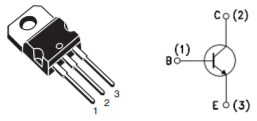
\includegraphics[width=6.8cm]{imagem/tip41c-w-schematic.png} 
    \caption{Transistor TIP41C NPN e seu diagrama interno}
    \label{fig:tip41c-npn}
\end{figure}

\subsection{Protocolo MQTT}
MQTT é um protocolo de transporte de mensagens do tipo \textit{publish/subscribe}. Projetado para ser leve, aberto, simples e fácil de implementar, é ideal para ser utilizado em soluções com ambientes limitados em hardware e software, para contextos de comunicação de máquina-a-máquina (M2M) e Internet das Coisas (IoT), onde memória e largura de banda são normalmente bastante limitados \cite{mqtt}.

Neste projeto, o protocolo MQTT é a base da comunicação entre as unidades, pois as leituras dos níveis dos contêineres são publicadas em um tópico específico, enquanto que o monitoramento, inscrito neste mesmo tópico, é capaz de obter e apresentar os dados para o operador, além de comandar o acionamento da unidade de escoamento conforme parâmetros pré-determinados. Da mesma forma, as unidades de escoamento, recebem informações sobre quando e o quanto escoar diretamente das unidades de monitoramento.

\subsection{Plataforma Node-RED}
Node-RED é uma plataforma low-code \cite{ibm-lowcode} para o desenvolvimento de aplicações baseadas em eventos \cite{nodered}, com uma interface baseada em \textit{nodes} (nós) que representam dispositivos e serviços, e através da interligação visual destes nodes é possível definir diversos tipos de fluxos que definem as funcionalidades das aplicações.

Com base na plataforma Node-RED, foi experimentado estender as funcionalidades propostas neste projeto, e como prova de conceito, foi implementado o monitoramento via navegador (\textit{browser}) com armazenamento dos dados das leituras dos sensores ultrassônicos em banco de dados relacional.

\subsection{RDBMS PostgreSQL}
PostgreSQL é um poderoso sistema de banco de dados relacional de objeto de código aberto com mais de 35 anos de desenvolvimento ativo que lhe rendeu uma forte reputação de confiabilidade, robustez de recursos e desempenho \cite{postgresql}.

Neste projeto, os dados lidos dos sensores ultrassônicos são gravados em um banco de dados PostgreSQL possibilitando a apresentação do histórico de variação dos níveis dos contêineres monitorados.

\clearpage